%%%%%%%%%%%%%%%%%%%%%%%%%%%%%%%%%%%%%%%%%%%%%%%%%%%%%%%%%%%%%%%%%%%%%%%%%%%%
\documentclass[a4j]{jarticle}

\usepackage{jsaisig}
% \usepackage{graphicx}
\usepackage[dvipdfmx]{graphicx}
\usepackage{subfigure}
\usepackage{multirow}
% \usepackage{}

%%%%%%%%%%%%%%%%%%%%%%%%%%%%%%%%%%%%%%%%%%%%%%%%%%%%%%%%%%%%%%%%%%%%%%%%%%%

\begin{document}

% 和文タイトル
% \title{Find My Matesに向けた解法の提案と実機での性能評価}
\title{RoboCup@Homeタスク:Find My Matesに向けた解法の提案とロボット実機での性能評価}

% 英文タイトル
\etitle{Solving RoboCup@Home Task: Find My Mates and evaluate on Domestic Standard Robot.}

% 著者名:
%	・各著者を\quad(全角空白)区切りで列挙
% 	・著者名の直後に\afil{所属番号}を追加→所属番号を上付で出力(\textsuperscript{所属番号}と同じ)
% 	 複数機関へ所属している場合は番号をカンマ区切りで列挙(下記著者2参照)
%  ・Corresponding Authorについては所属の後に\thanksを続け,連絡先を記入
%	・英文著者はカンマ区切りで列挙

\author{矢野 優雅\afil{1}%
	\thanks{連絡先:九州工業大学大学院生命体工学研究科人間知能システム工学専攻 \newline%
		      〒808-0135 福岡県北九州市若松区ひびきの2-4 \newline%
		      E-mail: yano.yuuga158@mail.kyutech.jp}\quad%
	松本 生弥\afil{1}
	福田 有輝也\afil{1}
	小野 智寛\afil{1}
	田向 権\afil{1,2}\\
	Yuga Yano\afil{1}, Ikuya Matsumoto\afil{1}, Yukiya Fukuda\afil{1}, Tomohiro Ono\afil{1}, and Hakaru Tamukoh\afil{1,2}}

% 所属
\affiliation{%
	\afil{1} 九州工業大学大学院生命体工学研究科\\
	\afil{1} Graduate School of Life Science and Systems Engineering, Kyushu Institute of Technology, Japan\\
	\afil{2} ニューロモルフィックAIハードウェア研究センター\\
	\afil{2} Research Center for Neuromorphic AI Hardware, Kyushu Institute of Technology, Japan}

\abstract{
% Abstract (English) comes here.......................................................
ホームサービスロボットの技術発展を目的として,RoboCup@Homeという競技会が開催されている.
RoboCup@Homeでは,実際の家庭環境を模したフィールドを用いてタスクを行うことで,より現実に近い環境でロボットの性能を評価することができる.
本研究では,RoboCup@Homeのタスクの一つであるFind My Matesに向けて,満点を取得するための手法を提案する.
% また,提案した手法をロボットに実装し,2022年7月にバンコクで行われたRoboCup@Homeにて現地実験を行った.
また,提案した手法をロボットに実装し,RoboCup@Homeにて現地実験を行った.
現地実験では満点を取得し,提案手法の有効性を示した.
% 現地実験の様子は,https://www.youtube.com/watch?v=Kh_eAm3_ZVw に公開している.
}

\maketitle
\thispagestyle{empty}

%%%%%%%%%%%%%%%%%%%%%%%%%%%%%%%%%%%%%%

\section{序論}
% テストと競技表記ゆれが起きそうなので,早いうちに確定させる
% \subsection{RoboCup@Home}
RoboCup@Home\cite{robocup_hp}は,ホームサービスロボットの技術発展を目的に開催されている競技会である.
本競技会では,人間とロボットの協調を目標の一つに掲げており,
音声認識や物体認識,ナビゲーションといったテストが動的環境下で行われている.
そのため,より現実に近い家庭環境で性能を評価することができ,非常に注目を集めているリーグとなっている.
% The RoboCup@Home league aims to develop service and assistive robot technology with high relevance for future personal domestic applications. It is the largest international annual competition for autonomous service robots and is part of the RoboCup initiative. A set of benchmark tests is used to evaluate the robots’ abilities and performance in a realistic non-standardized home environment setting. Focus lies on the following domains but is not limited to: Human-Robot-Interaction and Cooperation, Navigation and Mapping in dynamic environments, Computer Vision and Object Recognition under natural light conditions, Object Manipulation, Adaptive Behaviors, Behavior Integration, Ambient Intelligence, Standardization and System Integration. It is colocated with the RoboCup symposium.
RoboCup@Homeには,Open Platform League,Domestic Standard Platform League(DSPL),Social Standard Platform Leagueという3つのリーグがある.
私たちの参加しているDSPLでは,トヨタ社が開発したHuman Support Robot(HSR)\cite{hsr_paper}を標準機に採用しテストを行っている.
図\ref{overview_hsr}に,HSRの外観と搭載されているデバイスを示す.
\begin{figure}[ht]
  \centering
  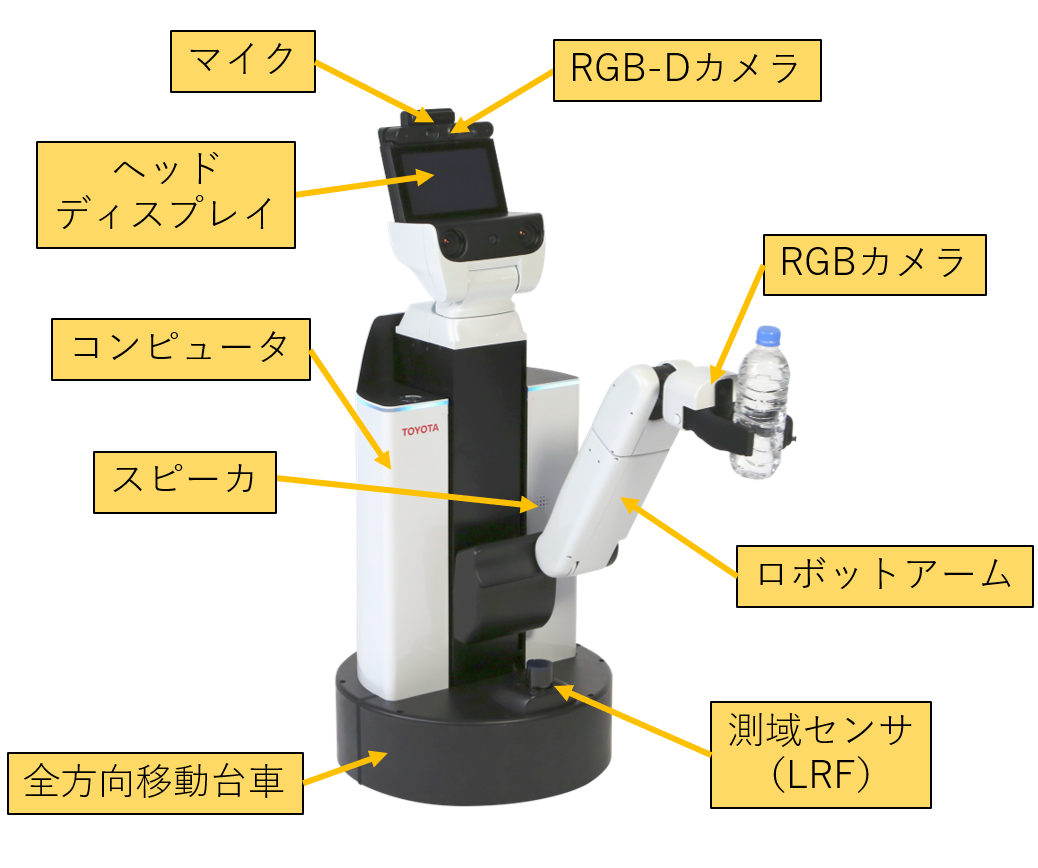
\includegraphics[width=6cm]{images/hsr/hsr_explain_ja.png}
  \caption{トヨタ社が開発したHSR}
  \label{overview_hsr}
\end{figure}
% HSRは移動台車やアームに加えて,RGB-Dカメラやマイクが搭載されており,認識を通して多様なヒューマンインタラクションを行うことができる.
HSRは移動台車やアームに加えて,RGB-Dカメラやマイクが搭載されているため,物体認識や音声認識を通して動的環境下においても多様な動作を実現できるロボットである.

本研究では,特にヒューマンインタラクションの性能をはかるFind My Mates(FMM)というテストに向けて,その解法を提案する.
また,提案した手法をHSRに実装し,2022年7月にバンコクで行われたRoboCup@Homeにて性能評価を行った.
現地実験では満点を取得し,本手法の有効性を示した.
しかし,課題も多く見つかったため,それらに対する考察も行う.
% RoboCup@Homeのタスクの一つであるFind My Mates(FMM)に着目する.
% FMMは人物認識や音声認識が必要となるタスクであり,特にヒューマンインタラクションの性能をはかることができる.

% 2ページ目の先頭に持ってくるため
\begin{figure*}[ht]
  \centering
  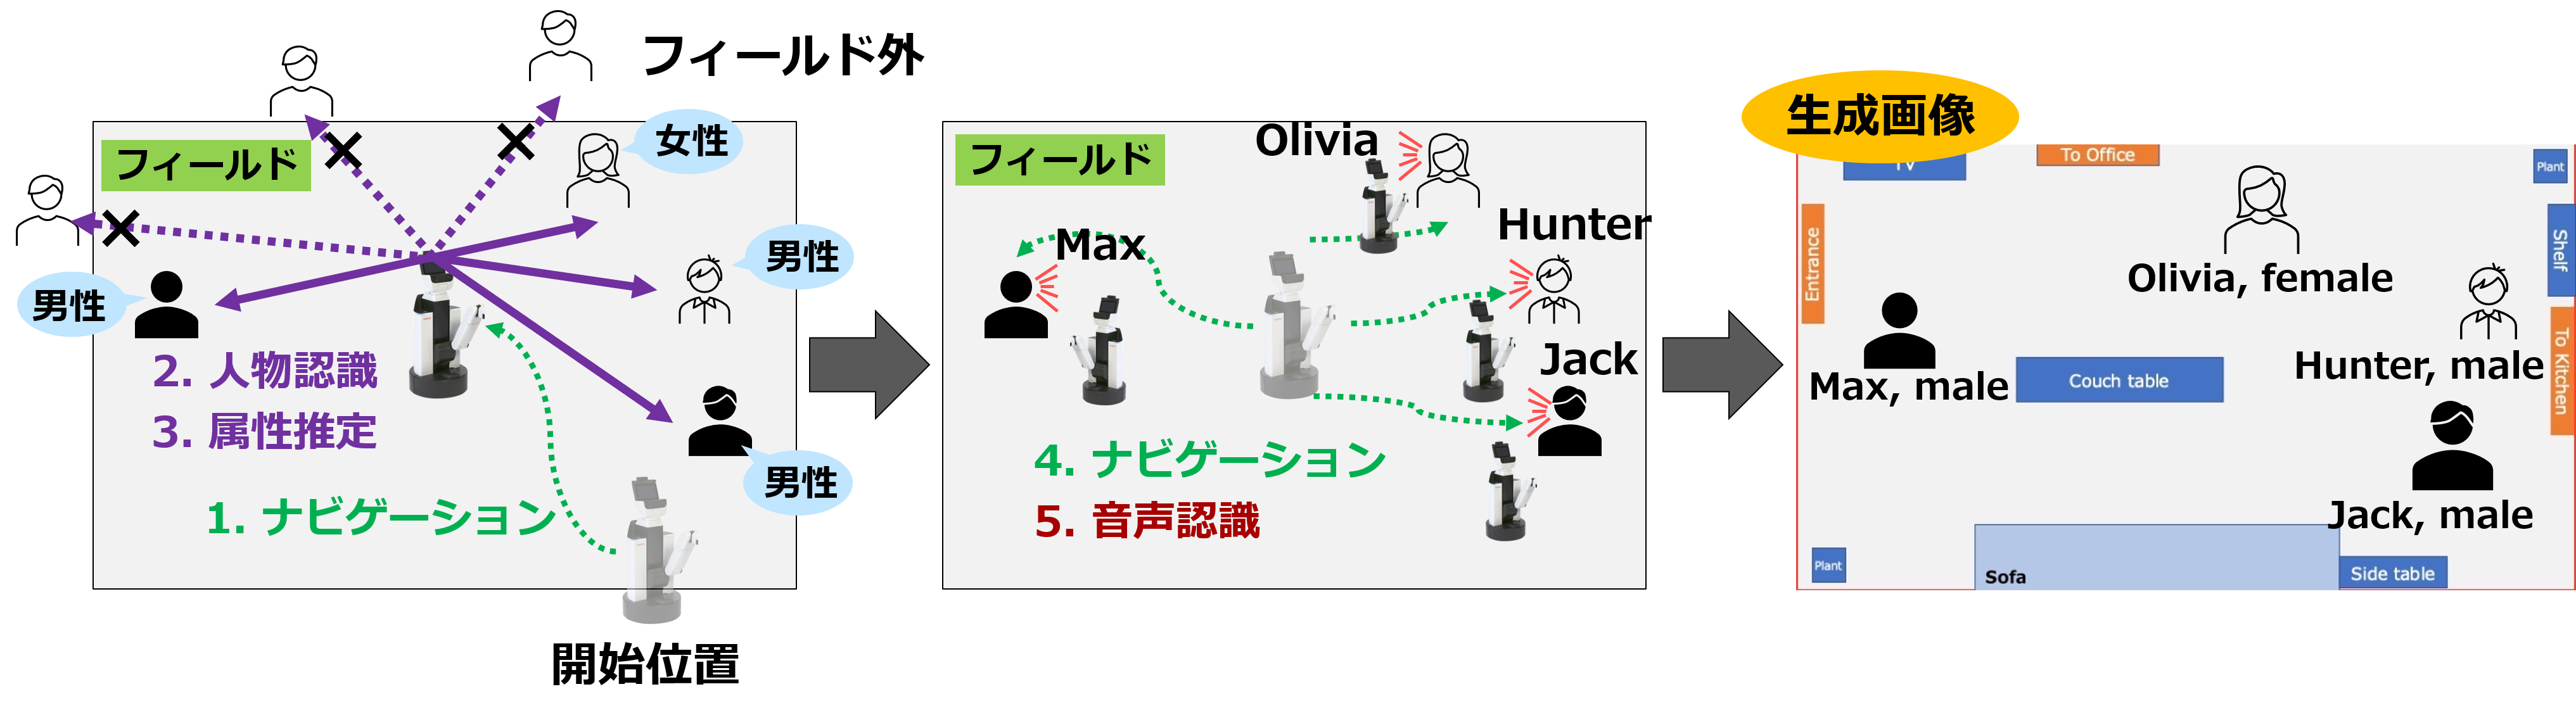
\includegraphics[width=16cm]{images/FMM/solution_overview_yoko_yy2.png}
  \caption{FMMの解法}
  \label{solution_overview}
\end{figure*}

% \subsection{Find My Mates}
% 本章では,RoboCup@Homeで行われるFind My Mates(FMM)というタスクについて述べる.
% FMMでは,4人のゲストが1人のホストを訪れたという状況を想定している.
% % しかし,ホストはゲストの名前のみを知っているがその他の情報は何も知らない.
% FMMは,1人のホストの家に訪れた4人のゲストをロボットが探し,その場所,名前に加えて人物の特徴をホストに報告するというタスクである.
% そのため,人物を3次元的に認識する技術と,それぞれのゲストの特徴を抽出する属性推定の技術が必要になる.
% 更に,ロボットは事前にゲストの名前を知らされていないため,音声認識を通してゲストの名前を知る必要がある.

% \section{RoboCup@Home}

\section{Find My Mates}
本節では,RoboCup@Homeで行われるタスクの一つであるFMMについて述べる.
FMMでは4人のゲストと1人のホストが登場し,ホストの家にゲスト全員が訪れたという状況を想定している.
しかし本タスクでは,ホストはゲストの名前のみを事前に知らされているが,それぞれの外見や特徴については何も知らされていない.
そのため,ロボットは家に訪れたゲストを見つけ出し,顔や特徴,また部屋のどこにいるのかをホストに伝える必要がある.

本タスクを遂行するためには,3次元位置を含む人物認識に加えて,人物の特徴を推定する技術が必要になる.
また,ゲストの名前を取得するためには,音声認識の技術も不可欠である.
% FMMにおける,評価項目と点数を表\ref{points_table_fmm}に示す.
% \begin{table}[]
% 	\centering
% 	\caption{FMMの得点表}
% 	\label{points_table_fmm}
% 	\begin{tabular}{cccc}
% 		\hline
% 		動作項目                    & 評価回数 & 1回あたりの評価点    & 合計評価点 \\ \hline \hline
% 		\multicolumn{4}{c}{\textbf{メインゴール}}                   \\ \hline
% 		ゲストの位置報告                & 2    & 100          & 200   \\ \hline
% 		位置の説明で,特定の一点のみを指し示せているか & 2    & 50           & 100   \\ \hline
% 		ゲストの説明を行う               & 2    & 150          & 300   \\ \hline
% 		\multicolumn{4}{c}{\textbf{ボーナス得点}}                   \\ \hline \hline
% 		3人目のゲストも報告できているか        & 1    & \textbf{150} & 150   \\ \hline
% 		3人目のゲストの特徴も報告できているか     & 1    & 250          & 250   \\ \hline
% 		\multicolumn{4}{c}{\textbf{減点対象}}                     \\ \hline \hline
% 		人物認識の際に,ゲストに合図を出してもらう   & 2    & -75          &       \\ \hline
% 		ゲストの位置を教えてもらう           & 2    & -75          &       \\ \hline
% 		ゲストがロボットの前方まで移動する       & 2    & -150         &       \\ \hline
% 		\multicolumn{3}{c}{合計}                        & 1000  \\ \hline
% 	\end{tabular}
% \end{table}

\begin{table}[]
	\centering
	\caption{FMMの得点表}
	\label{points_table_fmm}
	\begin{tabular}{cccc}
		\hline
		動作項目                                                       & 回数 & 点/回数         & 合計点  \\ \hline
		\multicolumn{4}{c}{\textbf{メインゴール}}                                                   \\ \hline
		ゲストの位置報告                                                   & 2  & 100          & 200  \\ \hline
		\begin{tabular}[c]{@{}c@{}}ユニークな特徴で\\ 位置を報告する\end{tabular} & 2  & 50           & 100  \\ \hline
		\begin{tabular}[c]{@{}c@{}}ゲストの\\ 特徴報告\end{tabular}        & 2  & 150          & 300  \\ \hline
		\multicolumn{4}{c}{\textbf{ボーナス得点}}                                                   \\ \hline
		\begin{tabular}[c]{@{}c@{}}3人目の\\ ゲストも報告\end{tabular}      & 1  & \textbf{150} & 150  \\ \hline
		\begin{tabular}[c]{@{}c@{}}3人目のゲストの\\ 特徴も報告\end{tabular}   & 1  & 250          & 250  \\ \hline
		\multicolumn{4}{c}{\textbf{減点対象}}                                                     \\ \hline
		\begin{tabular}[c]{@{}c@{}}ゲストから\\ 合図をもらう\end{tabular}     & 2  & -75          &      \\ \hline
		\begin{tabular}[c]{@{}c@{}}ゲストの位置を\\ 教えてもらう\end{tabular}   & 2  & -75          &      \\ \hline
		\begin{tabular}[c]{@{}c@{}}ゲストから\\ ロボットに近づく\end{tabular}   & 2  & -150         &      \\ \hline
		\multicolumn{3}{c}{合計}                                                         & 1000 \\ \hline
	\end{tabular}
\end{table}

\subsection{登場人物について}
\label{about_name_list}
RoboCup@Homeでは,タスクに登場する人物はボランティアから選出されるため,トライごとに変化する.
また,登場人物は自分の本名を使用するのではなく,事前に公開されている名前リストよりランダムに決定される.
この名前リストには,アメリカで一般的に使用されている名前から選出した男女11個ずつの名前が含まれている.
しかし,名前のみで男女の判別ができないように,男女で共通している名前が複数存在する.


\section{提案手法}
本章では,FMMで満点を取得する解法と,HSRに実装した機能について述べる.
% FMMでは部屋に移動した後,4人のゲストを見つける必要がある.

\subsection{FMMに向けた解法}
私達はFMMで満点を取得するために,次のような手法を提案する.
提案手法の概要を図\ref{solution_overview}に示す.
初めに,ロボットを部屋の中央までナビゲーションさせ,部屋全体を見渡しながら人物認識を行う.
人物の認識にはRGB画像を用いるが,Depth画像も用いることで,認識した人が部屋のどこにいるのかも同時に算出する.
% 次に,認識した人がエリア内のどこにいるかの判定を行う.これには,大きく2つの理由がある.
% 1つは,ロケーション報告に用いるためであり,
% もう1つは,フィールド周囲の観客の誤認識を防ぐためである.
算出した人物の位置情報を基に,各ゲストの正面までナビゲーションを行い,名前を聞く.
更に属性推定の手法を用いて,ゲストの性別を推定する.

最後に,取得したすべての情報(人物の画像,位置,名前,性別)を集約した1枚の画像を作成し,
ヘッドディスプレイに表示することでホストに伝える.

\subsection{音声認識}
近年ではスマートフォンやスマートスピーカーなどの普及により,クラウドを用いた音声認識の研究が盛んである.
しかし,RoboCup@Homeでは会場のネットワークが不安定である場合が想定され,安定したクラウド上での音声認識は困難である.
また,ネットワークの課題は一般の家庭環境においても想定されるものであるため,オフラインでの音声認識技術が必要である.
% を利用することは非常に有効である.
そこで本研究では,vosk\cite{vosk_hp}と呼ばれるオフライン音声認識手法を用いる.

本研究では,音声認識を次のように実装している.
まず,HSRのヘッド部に搭載されているマイクを用いて,音声認識を開始したタイミングから一定時間録音を行う.
次に,録音した音声をPC側へRobot Operating System(ROS)\cite{ros_wiki}を介して送信する.
しかし,ROSには音声ファイルをそのまま扱うメッセージ型がないため,本研究では音声ファイルをnumpy形式に変換して送信する.
% ここで,ROSには音声ファイルをそのまま送信できるメッセージ型がないため,音声ファイルをnumpyの配列に読み直して送信を行う.
PC側では,受信したnumpyの配列から音声ファイルを再構築し,音声認識を行う.
% 音声ファイルをROSで通信したことも書く.
% 音声認識を一定時間で行っていることも書く
% 音声認識の結果の評価があっても面白い
% 一回でも認識できなかったら,そのタスク中は音声認識をあきらめる事もかいておくべき

\subsubsection{辞書設定}
% RoboCup@Homeでは,タスクに登場する人物は本名を使用するのではなく,
% 事前に公開している名前リストから毎回ランダムに決定され名前を割り当てられる.
% この名前リストには,男性用と女性の用の名前が約10個ずつ用意されている.
% ただし,名前だけで性別の区別ができないようにするために,男性と女性で共通している名前も存在する.
第\ref{about_name_list}節で述べた通り,RoboCup@Homeではタスクに登場する人物の名前リストが公開されている.
そのため,本研究では名前リストを基にした辞書を作成し,voskに適用させることで音声認識の精度向上を図る.
% ここ定量的な表現に直す
辞書を設定していない場合では,名前を話してもまったく違う単語として認識されることがほとんどであったが,
辞書設定をすることで認識率は飛躍的に向上した.

\subsection{ノイズ除去}
RoboCup@Homeは実際の家庭環境を模したフィールドで行われるが,実際の家庭環境と異なる点もある.
その一つが,周囲の外音(ノイズ)が大きいことである.
RoboCup@Homeには多くの観客がおり,また他のリーグも同時に行われているため,実際の家庭環境では起きないような大きなノイズが発生する.
本研究では,音声認識の精度を高めるために,ノイズ除去\cite{sainburg2020finding}を音声認識の前段に組み込んでいる.
% これに定量的な実験結果を載せてもいいと思う

\subsection{音声認識の性能評価}
RoboCup@Homeで使用される名前は,アメリカで一般的に用いられる名前からランダムに決定される.
そこで,アメリカで一般的に使用されている名前から男女それぞれ名前を11個選出し,本研究で作成した音声認識の精度を検証した.
検証はノイズの大きな環境で行い,話者とノイズの環境を変化させながらそれぞれ4度ずつ読み上げて検証を行った.
% 検証データは

表\ref{voice_recognition_result}に,ノイズ除去を行った場合と辞書指定を行った場合における認識結果を示す.
辞書指定を行い,ノイズ除去を行った手法が最も精度が高くなっていることが確認できる.
\begin{table}[]
	\centering
	\caption{音声認識の精度}
	\begin{tabular}{|c|c|c|}
	\hline
	辞書指定                & ノイズ除去 & 認識精度(\%)          \\ \hline
	\multirow{2}{*}{なし} & なし    & 13.6          \\ \cline{2-3}
	                    & あり    & 10.2          \\ \hline
	\multirow{2}{*}{あり} & なし    & 69.3          \\ \cline{2-3}
	                    & あり    & \textbf{71.6} \\ \hline
	\end{tabular}
	\label{voice_recognition_result}
\end{table}

\subsection{人物認識}
本研究では人物認識の手法にLightweight Human Pose Estimation\cite{light-openpose}を用いた.
本手法は処理が非常に軽量であり,CPUでも高速に動作できる手法である.
% 今回使用したPCでは,x fpsで動作しており,HSRのカメラ周期と同等な速度である為,リアルタイム動作を実現できていると言える.
本手法を用いることで,図\ref{human_estimation_explain} (a)に示すように,HSRより取得したRGB画像から人物認識を行うことができる.
次に,RGB画像における認識結果と,Depth画像を合わせることで,人物の3次元位置推定を行う.
図\ref{human_estimation_explain} (b)に,人物の3次元位置推定を行った結果を示す.
% 本研究では,人物を3次元的に認識する必要があるため,RGB画像から人物認識を行った後,
% 認識位置のDepth画像を参照することで,3次元的な位置を推定する.
% 図\ref{human_estimation_explain}に,人物の3次元的な位置推定を行った結果を示す.
\begin{figure}[b]
  \centering
  \subfigure[RGB画像での認識結果]{
  	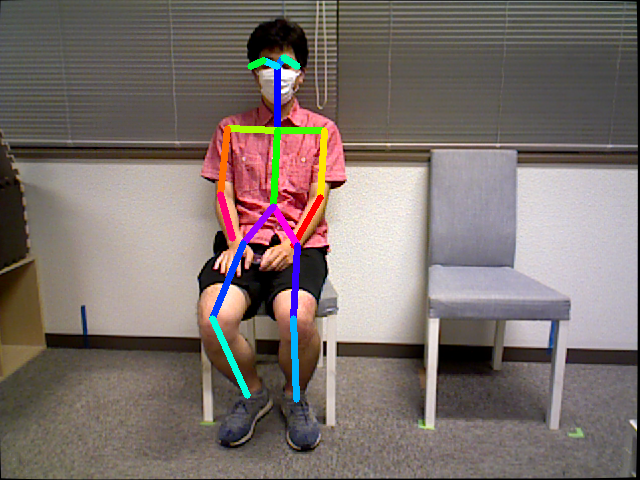
\includegraphics[height=3cm]{images/human_recognition/image.png}
	\label{human_estimation_image}
	% \caption{RGB画像での認識結果}
  }
  % \subfigure[Depth画像と合わせた3次元の位置推定]{
  \subfigure[3次元の位置推定]{
  	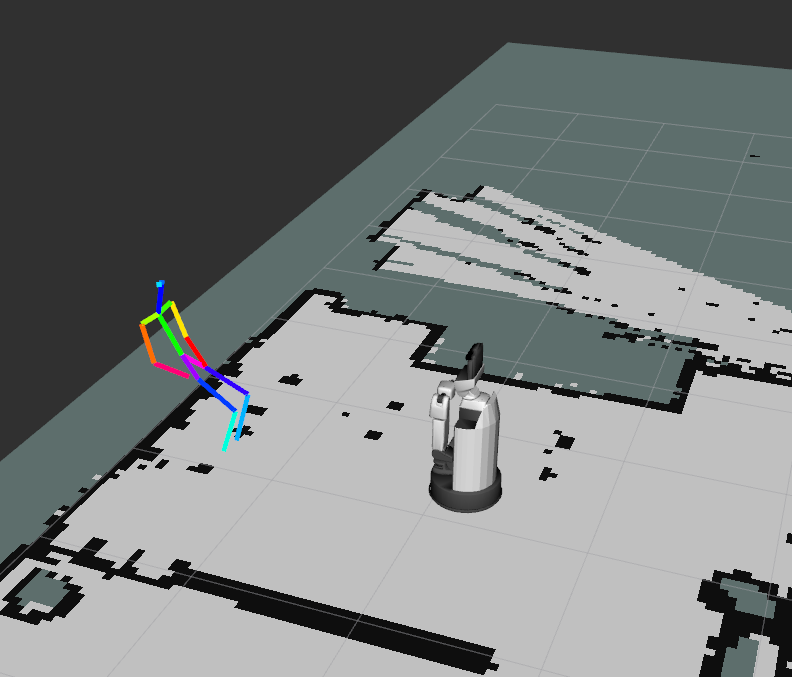
\includegraphics[height=3cm]{images/human_recognition/ss_4_trim.png}
	\label{human_estimation_pc}
	% \caption{Depth画像と合わせた3次元の位置推定}
  }
  \caption{人物位置推定アルゴリズム}
  \label{human_estimation_explain}
\end{figure}

\subsection{ゲストの位置報告}
FMMでは,認識した人物をホストに伝える必要があるが,この際に考慮すべきこととして,
認識した人が本当に部屋の中にいる人なのか,部屋の中のどこにいるのかを識別する必要がある.
そこで本研究では,事前に作成しているマップに対してjsonファイルを用いて意味づけを行い,フィールド内判定を行う.
またRoboCup@Homeでは,事前に部屋の形が公開されるため部屋の中のどこに椅子があるのかという意味づけも行う.
人物のフィールド内判定と,位置推定の結果を図\ref{human_where_map}に示す.
\begin{figure}[ht]
  \centering
  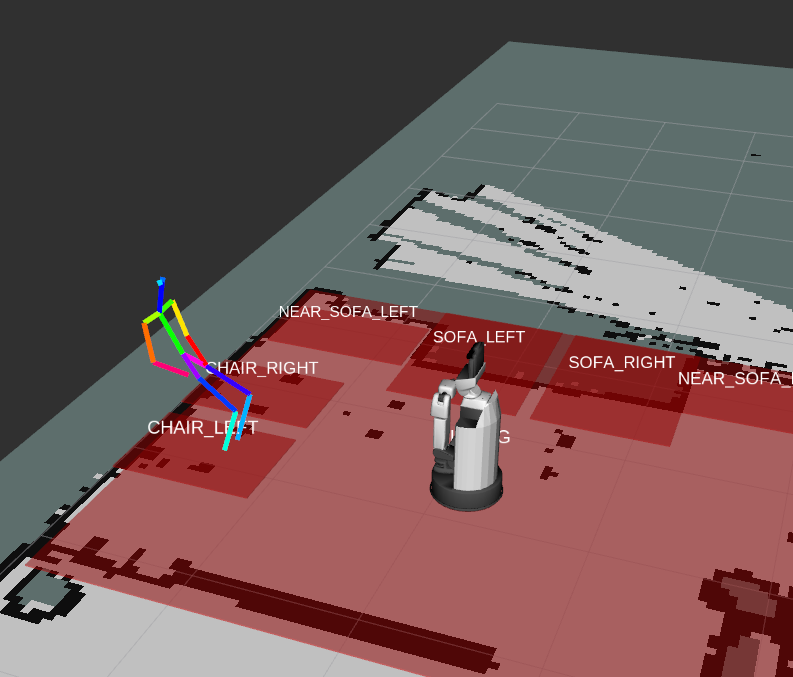
\includegraphics[width=6cm]{images/human_recognition/ss_5_trim.png}
  \caption{図\ref{human_estimation_explain}で認識した結果にエリア判定を付加した結果}
  \label{human_where_map}
\end{figure}
この場合では,ゲストはフィールド内の左側の椅子に座っており,それを正しく判定できている.

%%%%%%%%%%%%%%%%%%%%%%%%%%%%%%%%%%%%%%

\section{現地実験概要}
提案手法をHSRに実装し,2022年7月にバンコクで行われたRoboCup@Homeで性能評価を行った.
図\ref{robocup_field}に,実際に使用されたフィールドを示す.
% RoboCup@HomeのDSPLでは,HSRにPCを接続して使用することが認められている.
\begin{figure}[ht]
  \centering
  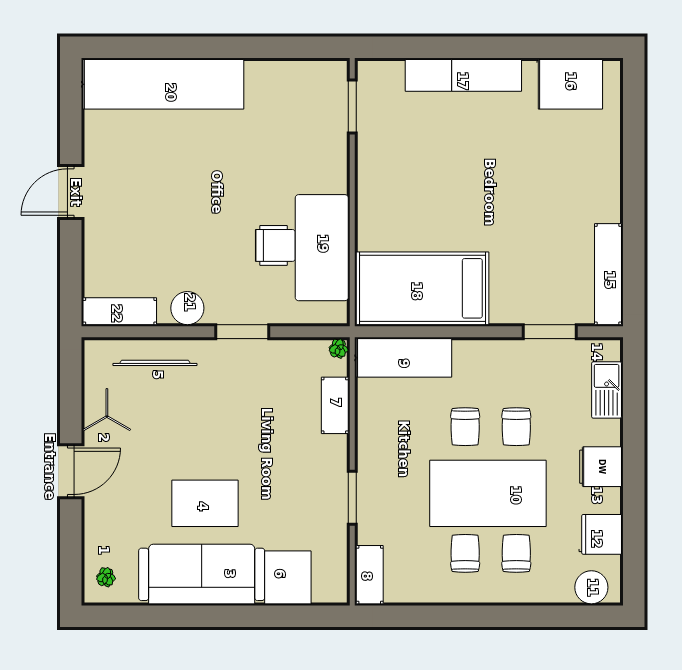
\includegraphics[width=6cm]{images/robocup/arenaBangkok_rotate.png}
  \caption{バンコクで開催されたRoboCup@Home2022で使用されたフィールド}
  \label{robocup_field}
\end{figure}
4つのルームがある中で,FMMはリビングルームにて実施された.
現地の実際の写真を図\ref{onsite_overview_1}に示す.
\begin{figure}[ht]
  \centering
  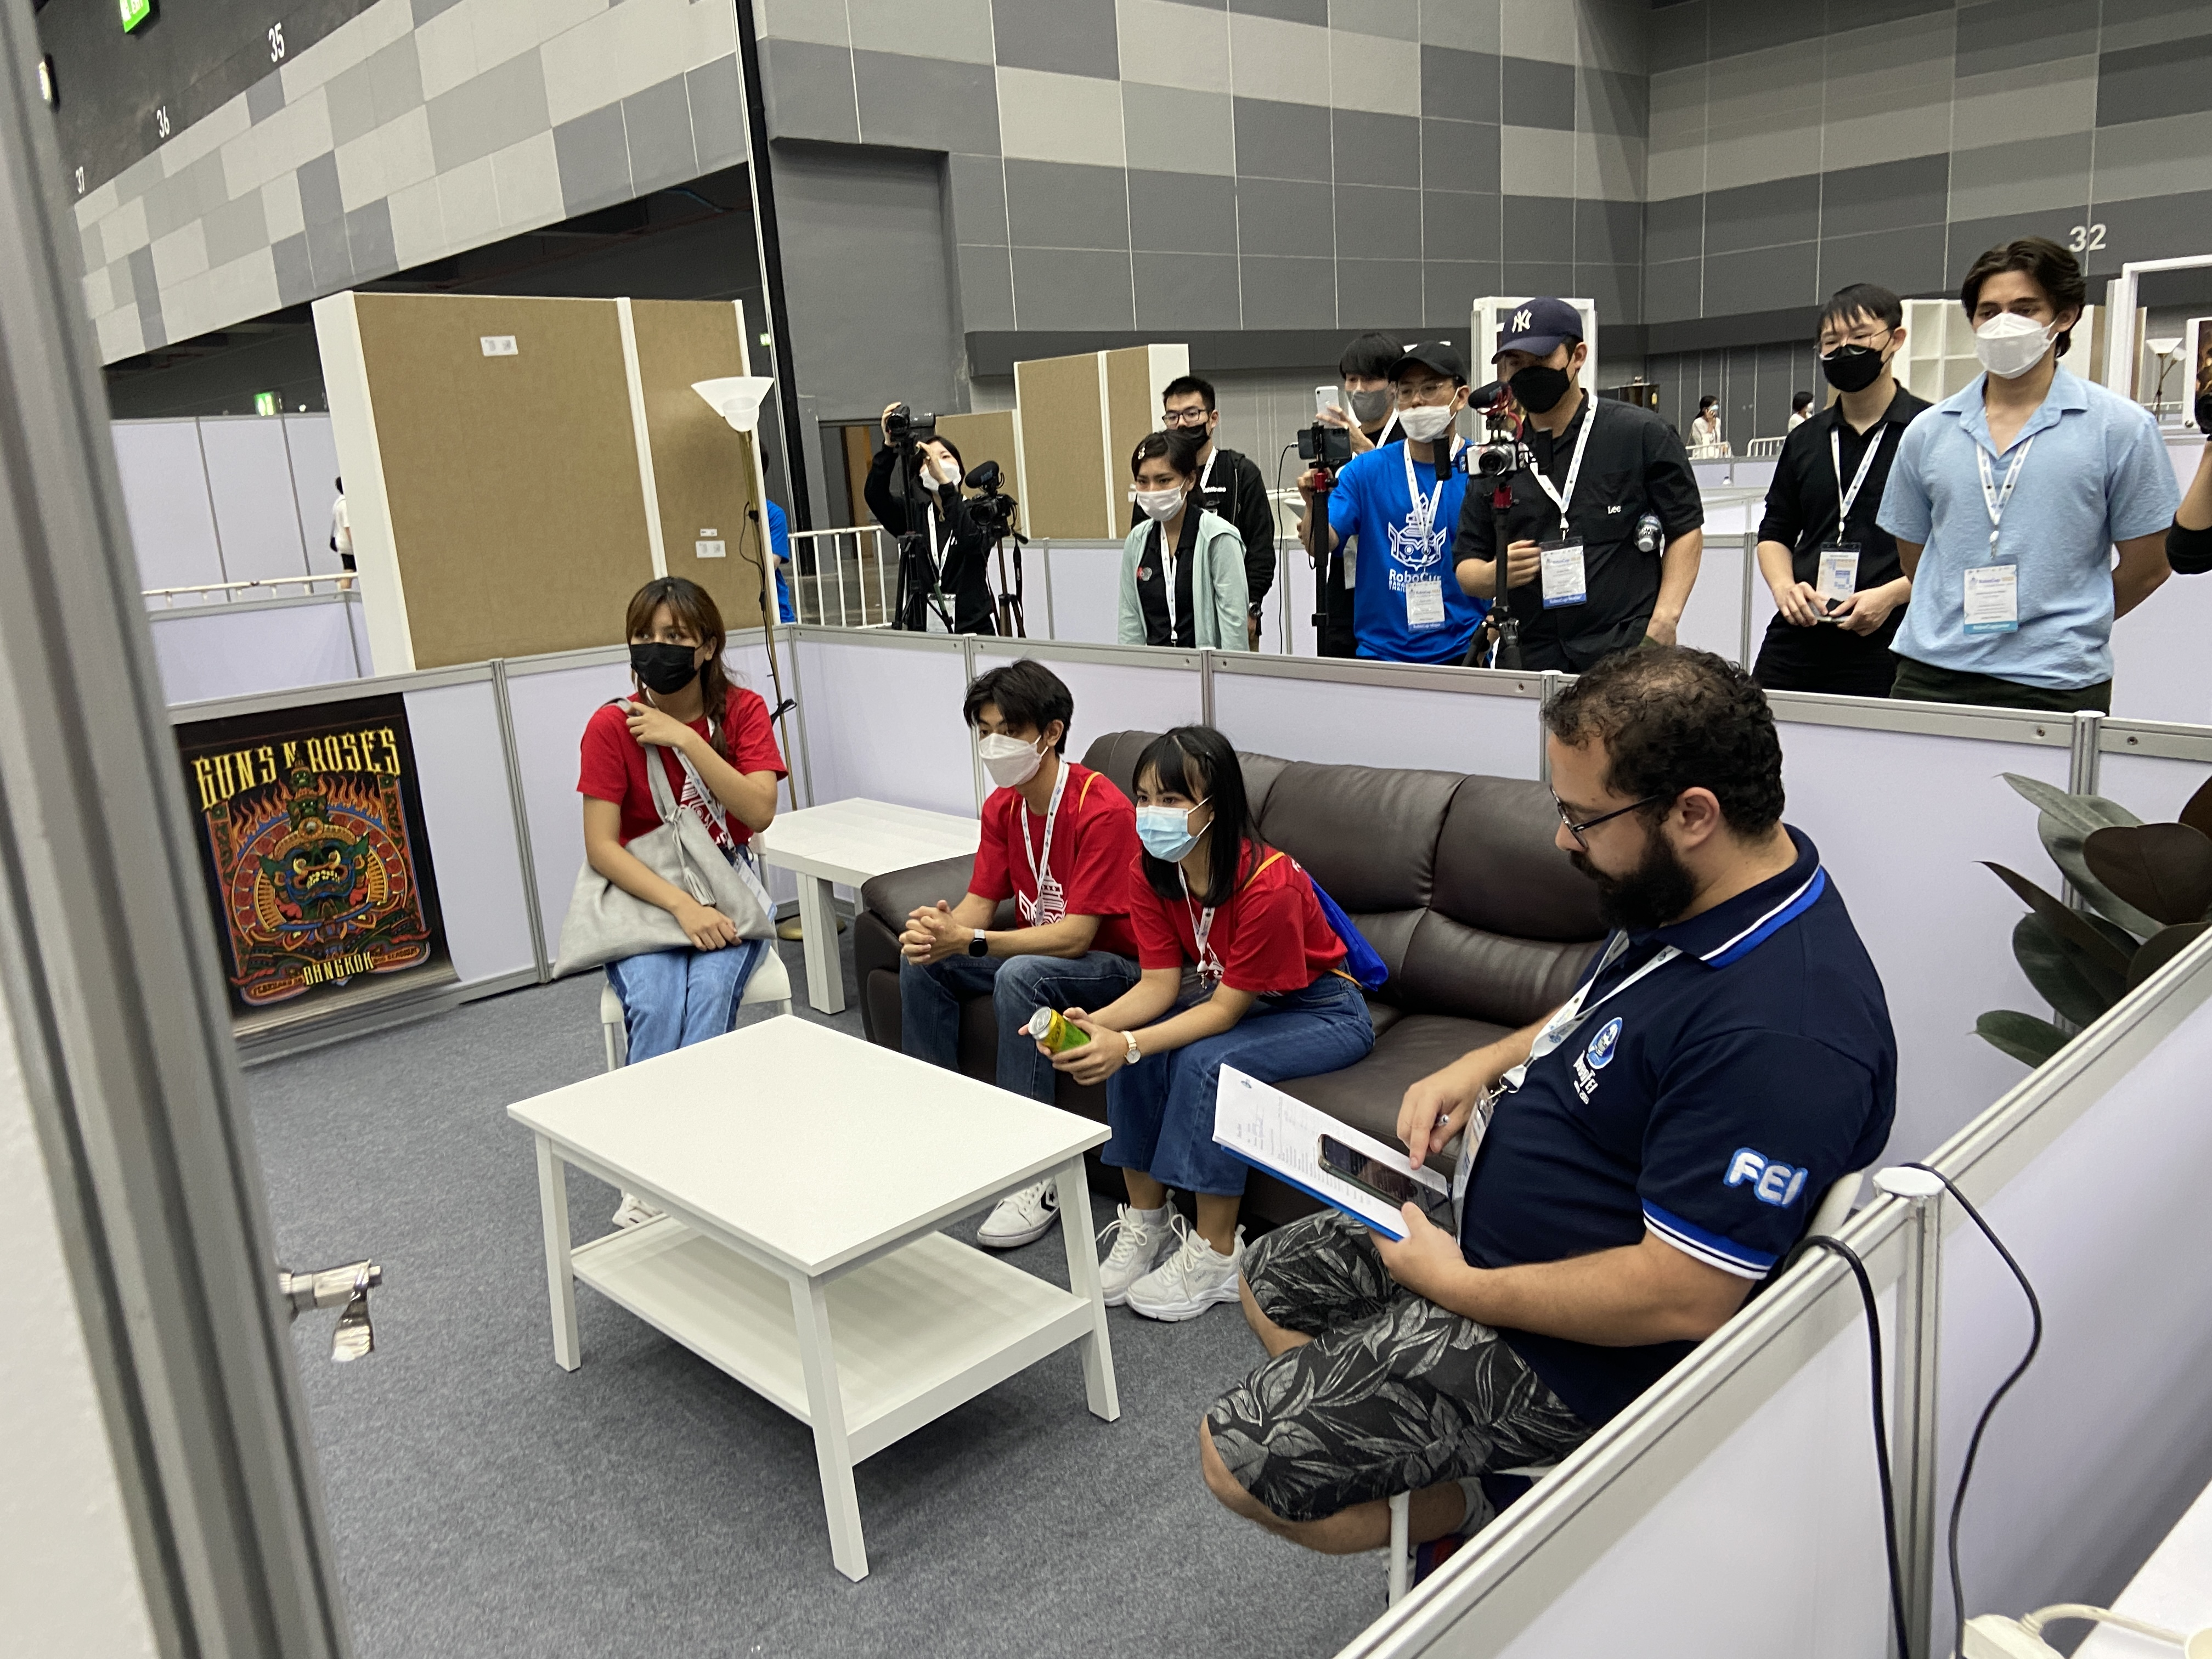
\includegraphics[height=2.2cm]{images/robocup/FMM_onsite_overview_1.jpg}
  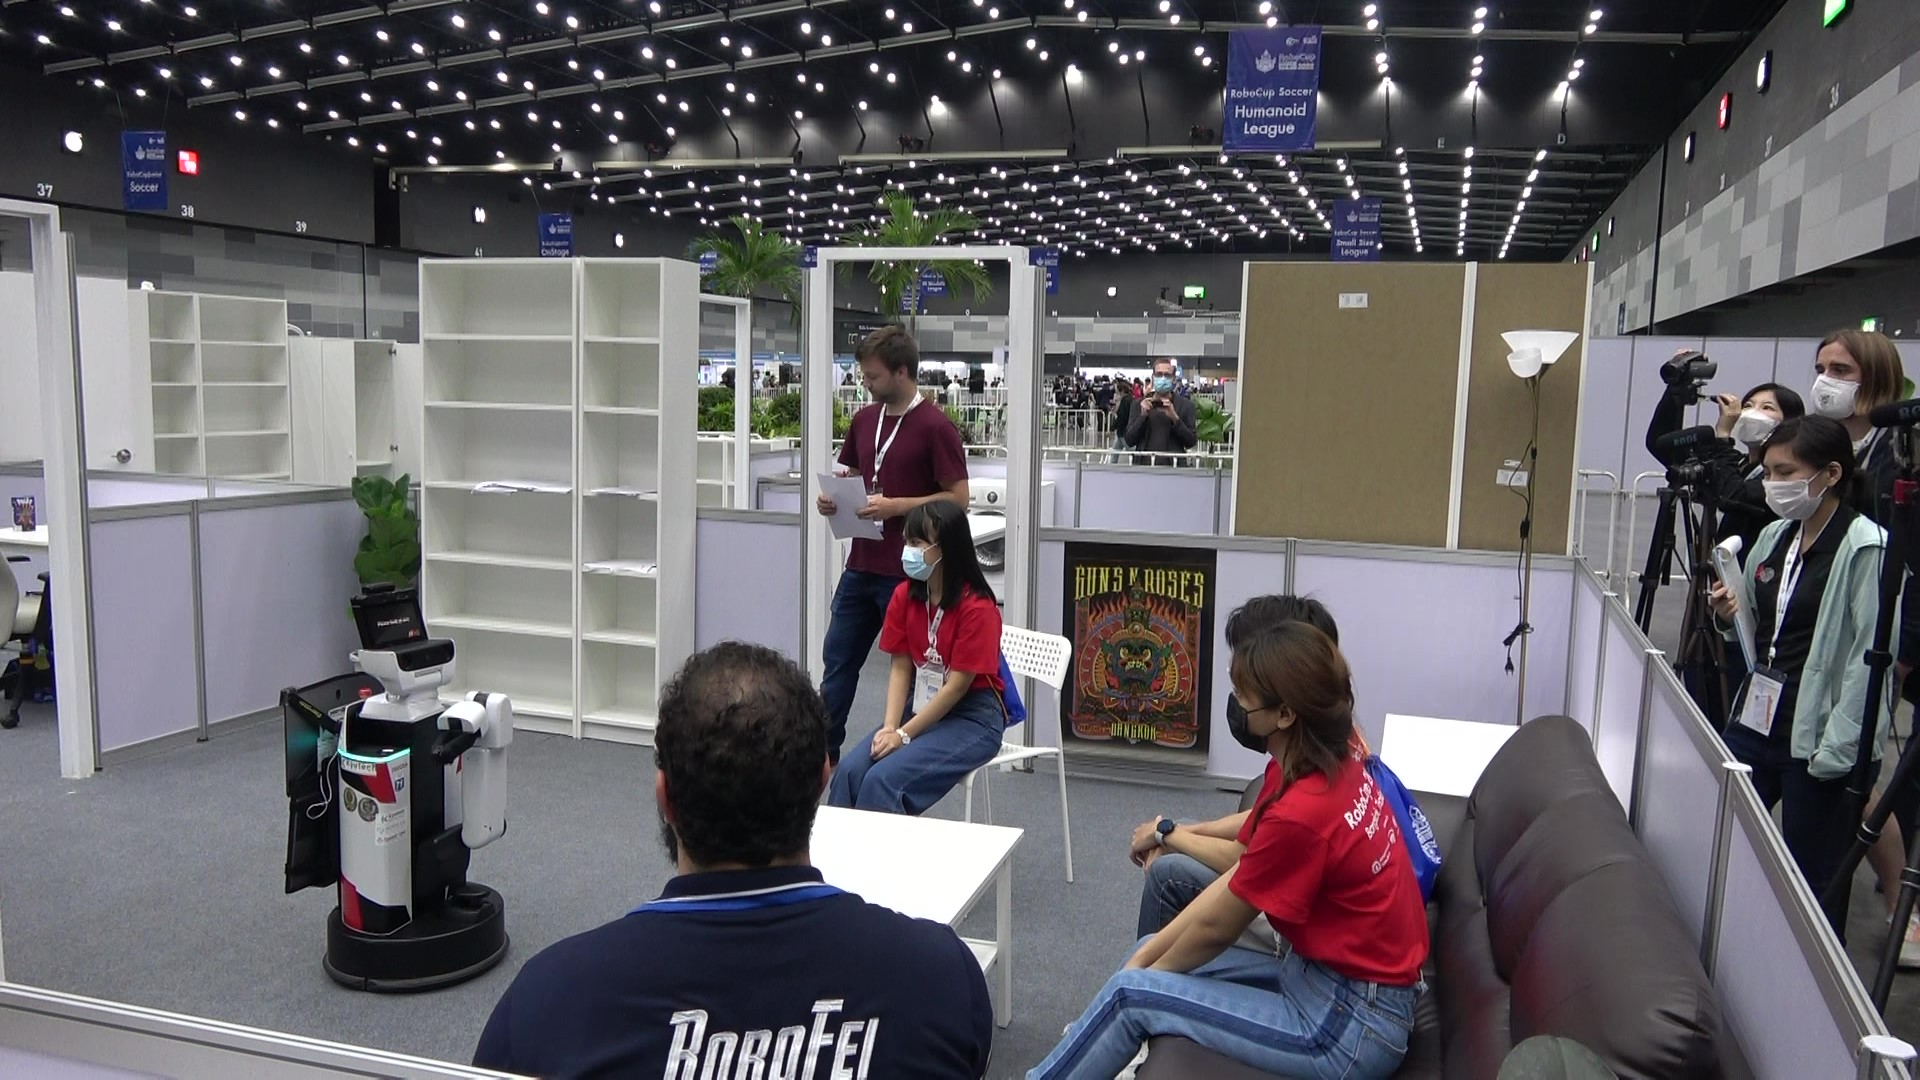
\includegraphics[height=2.2cm]{images/robocup/FMM_onsite_overview_3.jpg}
  \caption{FMMが行われた実際の会場}
  \label{onsite_overview_1}
\end{figure}

また,本研究で使用したPC環境は,CPU:Intel core, GPU:Geforce RTX 1080,メモリ:64GB,OS:Ubuntu18.04である.

\section{現地実験結果}
\subsection{実験結果}
私たちはRoboCup@HomeでFMMを2度トライし,性能評価を行った.
1度目のトライでは部屋中央へのナビゲーションに失敗し,ゲストから遠い位置にHSRが停止してしまった.
% の目的地がゲストから遠い位置であったため,
% その結果,不鮮明・不明瞭な画像を取得することとなった.
それでも,人物検出と3次元の位置推定は正常に動作したが,各ゲストの顔画像が非常に低い解像度となってしまった.
そのため属性推定が正常に動作せず,ゲストの2人が男性で2人が女性であったが,全員を女性と判定した.
また,音声認識では認識結果を得ることが出来ず,QRコードによるバイパスを用いた.
結果としては,ヘッドディスプレイに表示した人物画像が不明瞭であったため,人物報告,位置報告の両方が認められず0点であった.

% 2度目のトライは,1度目にあったナビゲーションの目的地が遠いという問題点を修正してから行った.
2度目のトライは,1度目にあったナビゲーションの問題点を修正してからトライした.
その結果,ゲストをより近い位置から認識することが出来たため,鮮明な画像を得ることができ,属性推定も間違いなく動作した.
しかし,音声認識部においてはゲストの前までナビゲーションを行うことは出来たが,名前を聞き取ることは出来ず,またQRコードのバイパスを使用することとなった.
2度目のトライにおいて,フィールド内の状況を説明するために生成した画像を図\ref{result_FMM_2}に示す.
\begin{figure}[ht]
  \centering
  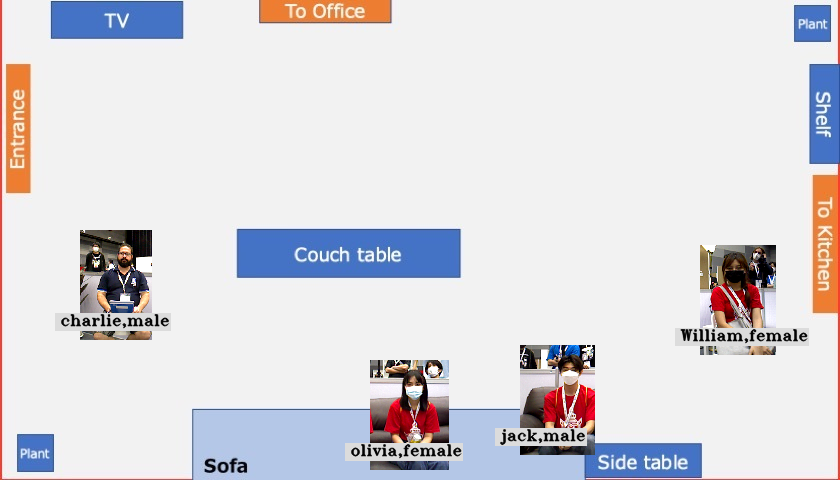
\includegraphics[width=7cm]{images/FMM/mapimage.png}
  \caption{2回目のトライで作成したマップイメージ}
  \label{result_FMM_2}
\end{figure}
今回のトライでは,ゲストは図\ref{robocup_field}の通りに座っており,生成画像では全員の座っている位置を間違いなく報告できている.
更に,性別と名前も正解しているため,結果として満点の1000点を取得した.
% 参加チームごとのFMMで取得した点数を表\ref{fmm_points_eachcheam}にまとめる.
% \begin{table}[h]
% \begin{tabular}{ll}
%                              & Find My Mates \\
% Hibikino-Musashi@Home (ours) & \textbf{1000} \\
% Tech United Eindhoven        & \textbf{1000} \\
% Team ORIon                   & 0
% \end{tabular}
% \label{fmm_points_eachcheam}
% \end{table}


\section{考察}

\subsection{音声認識について}
今回の現地実験では,FMMを2回実施したが,いずれも音声認識の結果を得ることは出来なかった.
% 原因として,音声認識中のGraphical User Interface(GUI)が発話者に伝わっておらず,音声認識時間外に発話されたことと,発話者の声量が小さく認識が困難であったことが考えられる.
1つ目の原因として,音声認識時間外に発話されたことが挙げられる.
まず,HSRはマイクとスピーカが別デバイスであるため,HSRが発話している間に音声認識を行うと,HSRの音声もマイクに入力されてしまう.
また,本研究で実装した音声認識は,ゲストの発話状態にかかわらず一定時間のみ行うため,発話のタイミングが音声認識の結果に大きく影響してしまう.
そこで,HSRのヘッドディスプレイに認識中を示すようなGUIを作成していたが,このGUIが発話者に伝わっておらず認識時間外に発話されることがあった.

2つ目の原因として,発話者の近くまでナビゲーションで移動出来なかったことが挙げられる.
バンコクで実際に使用された会場では,ゲストの座っているソファの手前にテーブルがあったため,ゲストの手前まで移動することが出来なかった.
そのため,遠い位置からの音声認識となり,マイクに入力される発話者の音声が非常に小さくなってしまった.
このことから,音声認識の結果を得ることが困難であったと考えられる.
今後は,発話のタイミングに応じて音声認識を開始,終了するような機能を作成する必要があると考える.
また,発話者の音声が小さいことも考慮して,音声強調\cite{voice_enhancement_1, voice_enhancement_2}の技術を活用する必要があると考える.

\subsection{位置推定について}
提案手法では,HSRが事前に取得したマップのどこがフィールドで,どこに椅子やソファがあるのかという情報を事前に与える必要がある.
RoboCup@Homeのルールでは,事前に部屋の情報が公開されることになっているが,本大会では椅子の位置が何度も変更されたため,対応が困難であった.
今後はロバスト性の高い3次元的な物体認識手法\cite{omni3d, sun2022onepose}を用いて,家具の位置変化に頑健なシステムを構築する必要があると考える.


\section{結論}
本研究では,国際的な競技会であるRoboCup@Homeで行われるFMMに向けての解法を提案し,実機実装を通してその性能評価を行った.
現地実験で,2回目のトライで満点を取得し,提案手法の有効性を示した.
一方で,音声認識やナビゲーションに関しての課題点も見つかったため,今後はこれらの課題を解決するために研究を続けていく必要がある.

\begin{thebibliography}{99}
%\small

\bibitem{robocup_hp}
RoboCup@Home. https://www.robocup.org/domains/3, (Accessed 2022-09-01).

\bibitem{hsr_paper}
% T. Yamamoto, K. Terada, A. Ochiai, F. Saito, Y. Asahara, and K. Murase, Development of Human Support Robot as the research platform of a domestic mobile manipulator, ROBOMECH Journal, Vol. 6, Art. no. 4, 2019.
Yamamoto, T., Terada, K., Ochiai, A., Saito, F., Asahara, Y., and Murase, K. “Development of Human Support Robot as the research platform of a domestic mobile manipulator,” ROBOMECH Journal, Vol. 6, Art. no. 4, (2019).

% \bibitem{vosk}
% Author, A., Author, B.:
% JSAI SIGs Conference Paper Format Sample,
% {\it International Journal of Examples}, Vol.~19, No.~4, pp.~1--2 (2007)

\bibitem{ros_wiki}
Robot Operating System Wiki. https://wiki.ros.org/, (Accessed 2022-09-01).

% \bibitem{yolo}
% 第一著者, 第二著者:
% 人工知能学会研究会原稿フォーマットサンプル,
% {\it International Journal of Examples}, Vol.~19, No.~4, pp.~1--2 (2007)

\bibitem{vosk_hp}
α cephei Vosk Offline speech recognition https://alphacephei.com/vosk/, (Accessed 2022-09-04).


\bibitem{sainburg2020finding}
Sainburg, T., Thielk, M., and Gentner, T. Q.,
% Sainburg, Tim and Thielk, Marvin and Gentner, Timothy Q
“Finding, visualizing, and quantifying latent structure across diverse animal vocal repertoires,”
{\it Public Library of Science PLoS computational biology},
Vol.16,
No.10,
pp.e1008228,
2020.

\bibitem{light-openpose}
Osokin, D. "Real-time 2d multi-person pose estimation on cpu: Lightweight openpose." arXiv preprint arXiv:1811.12004 (2018).
% Osokin, Daniil. "Real-time 2d multi-person pose estimation on cpu: Lightweight openpose." arXiv preprint arXiv:1811.12004 (2018).

\bibitem{voice_enhancement_1}
  % author = {Serrà, Joan and Pascual, Santiago and Pons, Jordi and Araz, R. Oguz and Scaini, Davide},
Serrà, J. and Pascual, S. and Pons, J. and Araz, R. O. and Scaini, D. “Universal Speech Enhancement with Score-based Diffusion,” arXiv (2022).

\bibitem{voice_enhancement_2}
% Simon Welker, Julius Richter and Timo Gerkmann. "Speech Enhancement with Score-Based Generative Models in the Complex STFT Domain", ISCA Interspeech, 2022.
Welker, S., Richter, J., and Gerkmann, T. "Speech Enhancement with Score-Based Generative Models in the Complex STFT Domain", ISCA Interspeech, (2022).

\bibitem{omni3d}
Garrick Brazil and Julian Straub and Nikhila Ravi and Justin Johnson and Georgia Gkioxari, “Omni3D: A Large Benchmark and Model for {3D} Object Detection in the Wild,” arXiv:2207.10660, (2022).

\bibitem{sun2022onepose}
Sun, Jiaming and Wang, Zihao and Zhang, Siyu and He, Xingyi and Zhao, Hongcheng and Zhang, Guofeng and Zhou, Xiaowei, “OnePose: One-Shot Object Pose Estimation without CAD Models,” Conference on Computer Vision and Pattern Recognition(CVPR), (2022).

\end{thebibliography}

\end{document}
